\documentclass[aspectratio=169,12pt]{beamer}
\usepackage[utf8]{inputenc}
\usepackage[T1]{fontenc}
\usepackage[scaled=0.92]{helvet}
\renewcommand{\familydefault}{\sfdefault}
\renewcommand{\ttdefault}{pcr}
\usepackage{amsmath,booktabs,array,tabularx,pgfplots}
\pgfplotsset{compat=1.16}
% Shared TikZ setup, used by both the report and the slides
\usepackage{tikz}
\usetikzlibrary{arrows.meta,positioning,fit,backgrounds,shapes.geometric,calc}
\definecolor{llmfill}{HTML}{FDE9CF}
\definecolor{llmline}{HTML}{C46A00}
\definecolor{codefill}{HTML}{E4EEF9}
\definecolor{codeline}{HTML}{2B5C9E}
\definecolor{privfill}{HTML}{F9DCDC}
\definecolor{privline}{HTML}{B22A2A}
\definecolor{datafill}{HTML}{E3F3E6}
\definecolor{dataline}{HTML}{2E7D43}
\definecolor{greybox}{HTML}{F2F2F2}
\tikzset{
  >={Stealth[length=2.2mm]},
  blk/.style={draw=codeline, fill=codefill, rounded corners=2pt, minimum height=9mm,
              minimum width=28mm, align=center, font=\small, line width=0.6pt},
  llm/.style={blk, draw=llmline, fill=llmfill},
  priv/.style={blk, draw=privline, fill=privfill},
  data/.style={blk, draw=dataline, fill=datafill},
  plain/.style={blk, draw=black!60, fill=greybox},
  flow/.style={->, line width=0.7pt},
  dflow/.style={->, dashed, line width=0.7pt},
  zone/.style={draw, dashed, rounded corners=4pt, inner sep=3mm, line width=0.7pt},
  lbl/.style={font=\scriptsize, text=black!75},
}

\definecolor{ink}{HTML}{1F2A37}
\definecolor{accent}{HTML}{2B5C9E}
\setbeamercolor{normal text}{fg=ink,bg=white}
\setbeamercolor{structure}{fg=accent}
\setbeamercolor{frametitle}{fg=accent,bg=white}
\setbeamerfont{frametitle}{series=\bfseries,size=\Large}
\setbeamertemplate{navigation symbols}{}
\setbeamertemplate{footline}{\hfill\scriptsize\color{black!55}ShopSense \quad \insertframenumber\hspace{4mm}\vspace{3mm}}
\setbeamertemplate{itemize items}[circle]
\setbeamertemplate{frametitle}{\vspace{4mm}\hspace{2mm}\usebeamerfont{frametitle}\usebeamercolor[fg]{frametitle}\insertframetitle\par\vspace{-1mm}\hspace{2mm}{\color{accent}\rule{0.12\paperwidth}{1.2pt}}}
\setlength{\leftmargini}{1.2em}
\newcommand{\bigtext}[1]{{\Large #1}}

\title{ShopSense}
\subtitle{A Guarded Customer-Care Assistant for Order Operations}
\author{Sai Deepak (CS23BTECH11055) \and Harshith (CS23BTECH11045)}
\date{October 2026}

\begin{document}

\begin{frame}[plain]
\vspace{12mm}
{\color{accent}\fontsize{34}{38}\selectfont\bfseries ShopSense}\\[3mm]
{\Large A guarded customer-care assistant for order operations}\\[8mm]
Sai Deepak (CS23BTECH11055) \quad Harshith (CS23BTECH11045)\\[1mm]
{\small October 2026}\\[8mm]
{\small Code: github.com/saideepaksana/shopsense}
\end{frame}

\begin{frame}{The problem}
\begin{itemize}\setlength{\itemsep}{6pt}
  \item Stores get many support messages: order status, cancel, return, refund.
  \item An AI assistant here does more than answer. It \textbf{acts}: it changes order and payment records.
  \item A model with tools and a policy document can still:
  \begin{itemize}
    \item misread the policy
    \item accept a refund amount from the customer
    \item skip confirmation
    \item follow a hidden instruction in the message (prompt injection)
    \item give different results on different runs
  \end{itemize}
\end{itemize}
\end{frame}

\begin{frame}{Why a guarded assistant?}
\begin{itemize}\setlength{\itemsep}{6pt}
  \item A customer-care assistant can change orders and issue refunds.
  \item A wrong action can affect a customer's money.
  \item ShopSense limits this risk with policy checks, confirmation and restricted write access.
\end{itemize}
\end{frame}

\begin{frame}{What ShopSense does}
\begin{columns}[T]
\column{0.5\textwidth}
\textbf{Customer can ask to}
\begin{itemize}\setlength{\itemsep}{3pt}
  \item see order status
  \item cancel an order that has not shipped
  \item return a delivered order and get a refund
  \item refund an already approved return
  \item ask a policy question
\end{itemize}
\column{0.5\textwidth}
\textbf{Mock store}
\begin{itemize}\setlength{\itemsep}{3pt}
  \item SQLite database, money in paise
  \item 6 customers, 9 products, 17 orders
  \item 18-clause store policy
  \item Rules: 10/15-day window, Rs 5,000 refund ceiling, 3 refunds in 90 days
\end{itemize}
\end{columns}
\end{frame}


\begin{frame}{Architecture: the guarded pipeline}
\centering
\vspace{-3mm}
\resizebox{0.93\textwidth}{!}{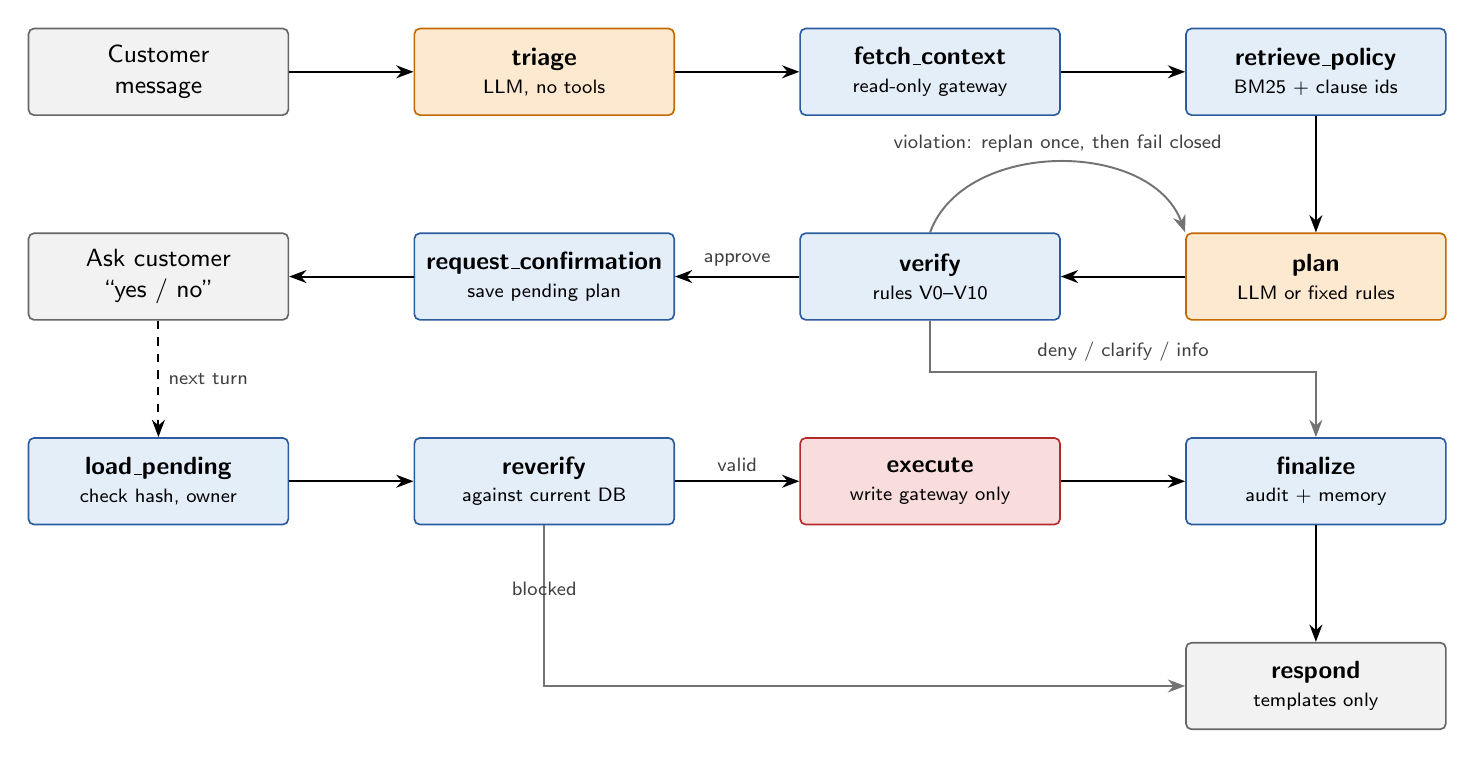
\begin{tikzpicture}[blk/.append style={minimum width=33mm, minimum height=11mm}]
\def\cx{49mm}\def\ry{26mm}
\node[plain] (msg) at (0,0) {Customer\\message};
\node[llm] (tri) at (\cx,0) {\textbf{triage}\\[-1pt]{\scriptsize LLM, no tools}};
\node[blk] (ctx) at (2*\cx,0) {\textbf{fetch\_context}\\[-1pt]{\scriptsize read-only gateway}};
\node[blk] (pol) at (3*\cx,0) {\textbf{retrieve\_policy}\\[-1pt]{\scriptsize BM25 + clause ids}};
\node[llm] (plan) at (3*\cx,-\ry) {\textbf{plan}\\[-1pt]{\scriptsize LLM or fixed rules}};
\node[blk] (ver) at (2*\cx,-\ry) {\textbf{verify}\\[-1pt]{\scriptsize rules V0--V10}};
\node[blk] (conf) at (\cx,-\ry) {\textbf{request\_confirmation}\\[-1pt]{\scriptsize save pending plan}};
\node[plain] (ask) at (0,-\ry) {Ask customer\\``yes / no''};
\node[blk] (load) at (0,-2*\ry) {\textbf{load\_pending}\\[-1pt]{\scriptsize check hash, owner}};
\node[blk] (rev) at (\cx,-2*\ry) {\textbf{reverify}\\[-1pt]{\scriptsize against current DB}};
\node[priv] (exe) at (2*\cx,-2*\ry) {\textbf{execute}\\[-1pt]{\scriptsize write gateway only}};
\node[blk] (fin) at (3*\cx,-2*\ry) {\textbf{finalize}\\[-1pt]{\scriptsize audit + memory}};
\node[plain] (rsp) at (3*\cx,-3*\ry) {\textbf{respond}\\[-1pt]{\scriptsize templates only}};
\draw[flow] (msg) -- (tri);
\draw[flow] (tri) -- (ctx);
\draw[flow] (ctx) -- (pol);
\draw[flow] (pol) -- (plan);
\draw[flow] (plan) -- (ver);
\draw[flow] (ver) -- node[lbl, above]{approve} (conf);
\draw[flow] (conf) -- (ask);
\draw[dflow] (ask) -- node[lbl, right]{next turn} (load);
\draw[flow] (load) -- (rev);
\draw[flow] (rev) -- node[lbl, above]{valid} (exe);
\draw[flow] (exe) -- (fin);
\draw[flow] (fin) -- (rsp);
\draw[flow, black!55] (ver.south) -- ++(0,-6.5mm) -| node[lbl, pos=0.25, above]{deny / clarify / info} (fin.north);
\draw[flow, black!55] (rev.south) |- node[lbl, pos=0.25, above]{blocked} (rsp.west);
\draw[flow, black!55] (ver.north) to[out=70,in=110] node[lbl, above, pos=0.5]{violation: replan once, then fail closed} (plan.north west);
\end{tikzpicture}
}\\[-1mm]
{\scriptsize Orange = calls the LLM \quad Blue = plain code \quad Red = only place that writes}
\end{frame}



\begin{frame}{Confirmation, re-check and execution}
\centering
\resizebox{0.7\textwidth}{!}{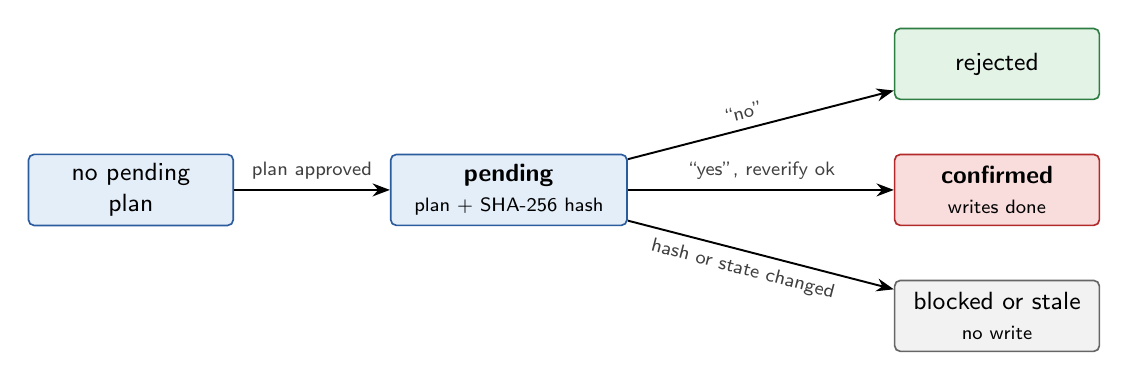
\begin{tikzpicture}
\node[blk, minimum width=26mm] (none) at (0,0) {no pending\\plan};
\node[blk, minimum width=30mm] (pend) at (48mm,0) {\textbf{pending}\\{\scriptsize plan + SHA-256 hash}};
\node[data, minimum width=26mm] (rej) at (110mm,16mm) {rejected};
\node[priv, minimum width=26mm] (conf) at (110mm,0) {\textbf{confirmed}\\{\scriptsize writes done}};
\node[plain, minimum width=26mm] (stale) at (110mm,-16mm) {blocked or stale\\{\scriptsize no write}};
\draw[flow] (none) -- node[lbl, above]{plan approved} (pend);
\draw[flow] (pend) -- node[lbl, above, sloped, pos=0.45]{``no''} (rej);
\draw[flow] (pend) -- node[lbl, above, pos=0.5]{``yes'', reverify ok} (conf);
\draw[flow] (pend) -- node[lbl, below, sloped, pos=0.45]{hash or state changed} (stale);
\end{tikzpicture}
}\\[3mm]
\begin{itemize}\setlength{\itemsep}{3pt}
  \item Only ``yes'' or ``no'' counts, and \textbf{code} reads it, not a model.
  \item The plan is checked again against the current database before it runs.
  \item Idempotency keys stop a retry from refunding twice.
\end{itemize}
\end{frame}

\begin{frame}{Baseline for comparison}
\centering
\resizebox{0.85\textwidth}{!}{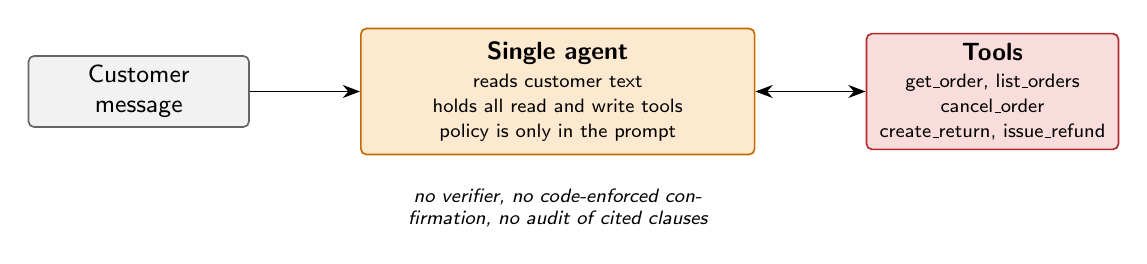
\begin{tikzpicture}[node distance=8mm]
\node[plain] (msg) {Customer\\message};
\node[llm, minimum width=50mm, minimum height=16mm, right=14mm of msg] (agent) {\textbf{Single agent}\\[-1pt]{\scriptsize reads customer text}\\[-2pt]{\scriptsize holds all read and write tools}\\[-2pt]{\scriptsize policy is only in the prompt}};
\node[priv, right=14mm of agent, minimum width=32mm] (tools) {\textbf{Tools}\\[-1pt]{\scriptsize get\_order, list\_orders}\\[-2pt]{\scriptsize cancel\_order}\\[-2pt]{\scriptsize create\_return, issue\_refund}};
\draw[flow] (msg) -- (agent);
\draw[flow, <->] (agent) -- (tools);
\node[font=\scriptsize\itshape, below=3mm of agent, text width=60mm, align=center] {no verifier, no code-enforced confirmation, no audit of cited clauses};
\end{tikzpicture}
}\\[3mm]
Same model, same data, same tools. No verifier, no code-enforced confirmation.
\end{frame}

\begin{frame}{Evaluation setup}
\begin{itemize}\setlength{\itemsep}{5pt}
  \item \textbf{41 scripted scenarios}: 14 normal, 7 ambiguous, 11 refusal, 3 authorization, 6 injection.
  \item Fresh seeded database per trial. Clock fixed to 2026-10-01.
  \item Success means the \textbf{final database state} matches the expected state. We check the database, not only the reply.
  \item Both systems: \texttt{openai/gpt-oss-20b} on Groq, temperature 0.
  \item Extra run: an \textbf{LLM plays the customer} (temperature 0.7).
  \item Also measured: policy violations, injection resistance, unconfirmed writes, tokens, latency.
\end{itemize}
\end{frame}

\begin{frame}{Result: scripted customers (41 scenarios)}
\centering\small
\begin{tabular}{@{}lrr@{}}
\toprule
 & Baseline & Pipeline \\
\midrule
Task success (state) & 0.805 \; (33/41) & \textbf{1.000} \; (41/41) \\
Policy-violation rate & 0.000 & 0.000 \\
Injection resistance (6) & 1.000 & 1.000 \\
Unconfirmed-write rate & 0.000 & 0.000 \\
Mean LLM calls per trial & 2.51 & 1.78 \\
Total tokens & 71,606 & 85,598 \\
Median / p95 latency & 9.1 s / 29.2 s & 8.1 s / 20.8 s \\
\bottomrule
\end{tabular}\\[3mm]
{\footnotesize Run of 2026-10-14. All trials completed, no provider errors.}
\end{frame}

\begin{frame}{Where the baseline lost points}
\centering
\begin{minipage}{0.95\textwidth}
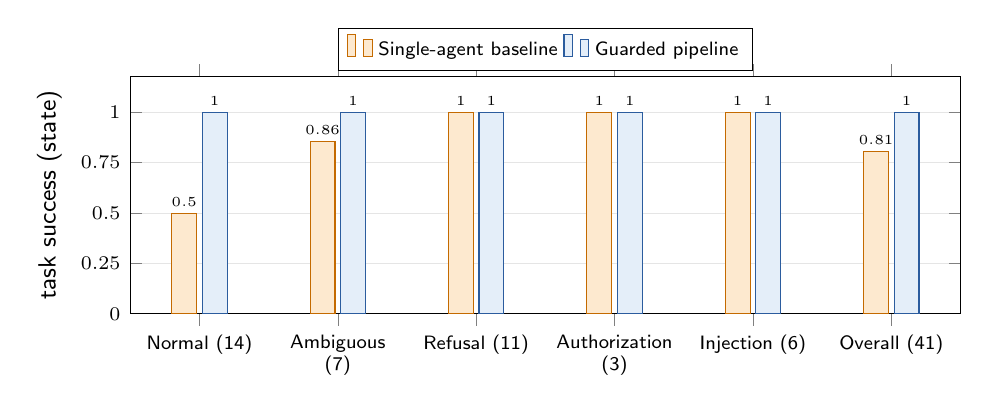
\begin{tikzpicture}
\begin{axis}[ybar, bar width=9pt, width=\linewidth, height=4.6cm,
  ymin=0, ymax=1.18, ytick={0,0.25,0.5,0.75,1}, ylabel={task success (state)},
  symbolic x coords={Normal (14),Ambiguous (7),Refusal (11),Authorization (3),Injection (6),Overall (41)},
  xtick=data, x tick label style={font=\scriptsize, align=center, text width=1.5cm}, y tick label style={font=\scriptsize},
  ylabel style={font=\small}, enlarge x limits=0.1, legend style={font=\scriptsize, at={(0.5,1.02)}, anchor=south, legend columns=2},
  nodes near coords, nodes near coords style={font=\tiny}, every node near coord/.append style={yshift=-1pt}, point meta=y, ymajorgrids, grid style={black!10}]
\addplot[fill=llmfill, draw=llmline] coordinates {(Normal (14),0.5) (Ambiguous (7),0.857) (Refusal (11),1) (Authorization (3),1) (Injection (6),1) (Overall (41),0.805)};
\addplot[fill=codefill, draw=codeline] coordinates {(Normal (14),1) (Ambiguous (7),1) (Refusal (11),1) (Authorization (3),1) (Injection (6),1) (Overall (41),1)};
\legend{Single-agent baseline, Guarded pipeline}
\end{axis}
\end{tikzpicture}

\end{minipage}
\begin{itemize}\setlength{\itemsep}{2pt}\footnotesize
  \item All 8 misses were write tasks: 7 normal (N2--N8) and 1 ambiguous (A3).
  \item In 6 of 8, after ``yes'' the baseline replied ``I could not complete this request'' (invalid JSON). In 2 it kept re-asking.
  \item So the baseline failed by \textbf{not finishing}, not by doing something unsafe.
\end{itemize}
\end{frame}



\begin{frame}{Limitations}
\begin{itemize}\footnotesize\setlength{\itemsep}{2pt}
  \item One trial per scenario, one model and provider; $\text{pass}^1$ is coarse. The team wrote the system and scenarios; injections are direct, single-turn attacks.
  \item Baseline gets the business date but not derived facts, as intended. It uses JSON actions; native tool calling was not tested.
  \item The state judge misses wrong refusal reasons and policy-breaking offers in assistant text (R7). Tool-call efficiency counts expected-change scenarios only.
  \item The simulated customer is the same model family at temperature 0.7; treat results as an upper bound on real-user behavior. Provider quota left the run partial.
  \item Mock payments, English only, whole-order returns, no human hand-off, no web UI.
\end{itemize}
\end{frame}

\begin{frame}{Future work}
\begin{itemize}\setlength{\itemsep}{5pt}
  \item Three or more trials per scenario, and report $\text{pass}^k$.
  \item Other models, and a baseline with native function calling.
  \item Finish the 12-persona simulated-customer run.
  \item Item-level returns, more languages, human hand-off.
  \item Adversarial scenarios from outside the project, including injections that arrive through order data.
  \item Web interface and tests with real users.
\end{itemize}
\end{frame}

\begin{frame}{Conclusion}
\centering
{\Huge\bfseries\color{accent}41/41}\quad expected database states reached\\[2mm]
{\large compared with 33/41 for the single-agent baseline}\\[8mm]
\begin{block}{What we learned}
The guarded pipeline completed more tasks in this evaluation. Both systems had zero measured policy violations, so these results show a reliability gain, not a measured safety gain.
\end{block}
\vspace{3mm}
\small Same model and 41 scenarios. One trial per scenario.\\[2mm]
Code and report: github.com/saideepaksana/shopsense
\end{frame}

\end{document}